\chapter{Power management}






%Il controller di potenza ha il compito di interfacciarsi con tutti i sensori fisici e gli attuatori, nonché con il sistema operativo e le applicazioni dell'utente. Grazie a queste interfacce, il controller di potenza legge periodicamente lo stato degli elementi di elaborazione principali (Processore, Temperatura e Tensione) e imposta di conseguenza, in base alle politiche di gestione della potenza, il punto di funzionamento di essi (Tensione, Frequenza). Oltre a queste metriche, il controller di potenza legge periodicamente il consumo energetico delle tensioni dei binari dal Resource Manager (RM) e riceve dall'OS le richieste in termini di livello di prestazioni (Frequenza Obiettivo), budget energetico e caratteristiche del carico di lavoro da eseguire. La politica di gestione della potenza determina, in base a questi parametri, il miglior punto di funzionamento in cui eseguire gli elementi di elaborazione, garantendo al contempo la stabilità termica, il budget energetico e i vincoli dell'applicazione. La gestione della potenza consente all'applicazione e al modello di programmazione in esecuzione di richiedere modifiche al punto di funzionamento in modo asincrono per seguire le fasi dell'applicazione ed entrare in punti di funzionamento a basso consumo energetico durante le fasi limitate dall'I/O, dalla memoria e dalla comunicazione per aumentare l'efficienza energetica.

\section{Stato dell'arte}

Come mostrato nella Figura 1, il controller di potenza è collegato: (i) on-chip ai controlli di potenza (gestendo il consumo energetico e le prestazioni degli elementi di elaborazione principali) e ai sensori (monitorando il processo, la temperatura e la tensione degli elementi di elaborazione principali); (ii) off-chip ai Moduli Regolatori di Tensione (VRM) che alimentano il chip, gli altri componenti a bordo e il Controller di Gestione della Scheda (BMC).

La gestione della potenza utilizza questi componenti hardware e connessioni per supportare un insieme di servizi in-band e out-of-band.

I servizi in-band vengono forniti alle applicazioni e ai sistemi operativi in esecuzione negli elementi di elaborazione del chip e sono composti da: (i) governor dedicati alla potenza e telemetria correlata alla potenza a livello di sistema operativo; (ii) un'interfaccia dedicata per consentire alle applicazioni e ai tempi di esecuzione del modello di programmazione di specificare suggerimenti e prescrizioni per la gestione della potenza; (iii) un'interfaccia dedicata al Sistema e alla Gestione delle Risorse per supportare il capping della potenza a livello di CPU e nodo, nonché per gestire il compromesso tra Throughput ed Efficienza Energetica. I servizi out-of-band vengono forniti all'amministratore di sistema e agli strumenti di gestione del sistema tramite il Controller di Gestione della Scheda (BMC). Questi servizi consistono nella telemetria di potenza out-of-band, nel capping di potenza a livello di sistema e nella affidabilità e assistenza.

\subsection{Servizi In-Band}
%\subsection{Interfacce SO}
Il Power Management condivide una regione di memoria interna con lo spazio degli indirizzi I/O degli elementi di elaborazione. Questa interfaccia consente all'OS di accedere periodicamente a un insieme di strutture dati di stato contenenti lo stato del controller di potenza, le statistiche e il consumo energetico dei diversi binari di tensione e componenti. Queste informazioni possono essere utilizzate e accessibili dalle applicazioni e dagli utenti per monitorare in modo dettagliato l'energia consumata dalle applicazioni, consentendo la consapevolezza energetica.

\subsection{Servizi Out-of-Band}
%\subsection{Board Management COntroller}
Oltre alla politica di gestione della potenza e ai servizi In-Band, il controller di potenza si interfaccia con il BMC per supportare servizi Out-of-Band. Questi includono la telemetria dettagliata sullo stato di potenza e prestazioni del chip, il capping di potenza a livello di chip e a livello di sistema e la segnalazione di errori e guasti nel chip e nei processi principali.

\subsection{Interfacce di alto livello}
%TODO
% slide 3-4 presentazione

\section{Componenti PowerStack}
\begin{figure}
    \centering
    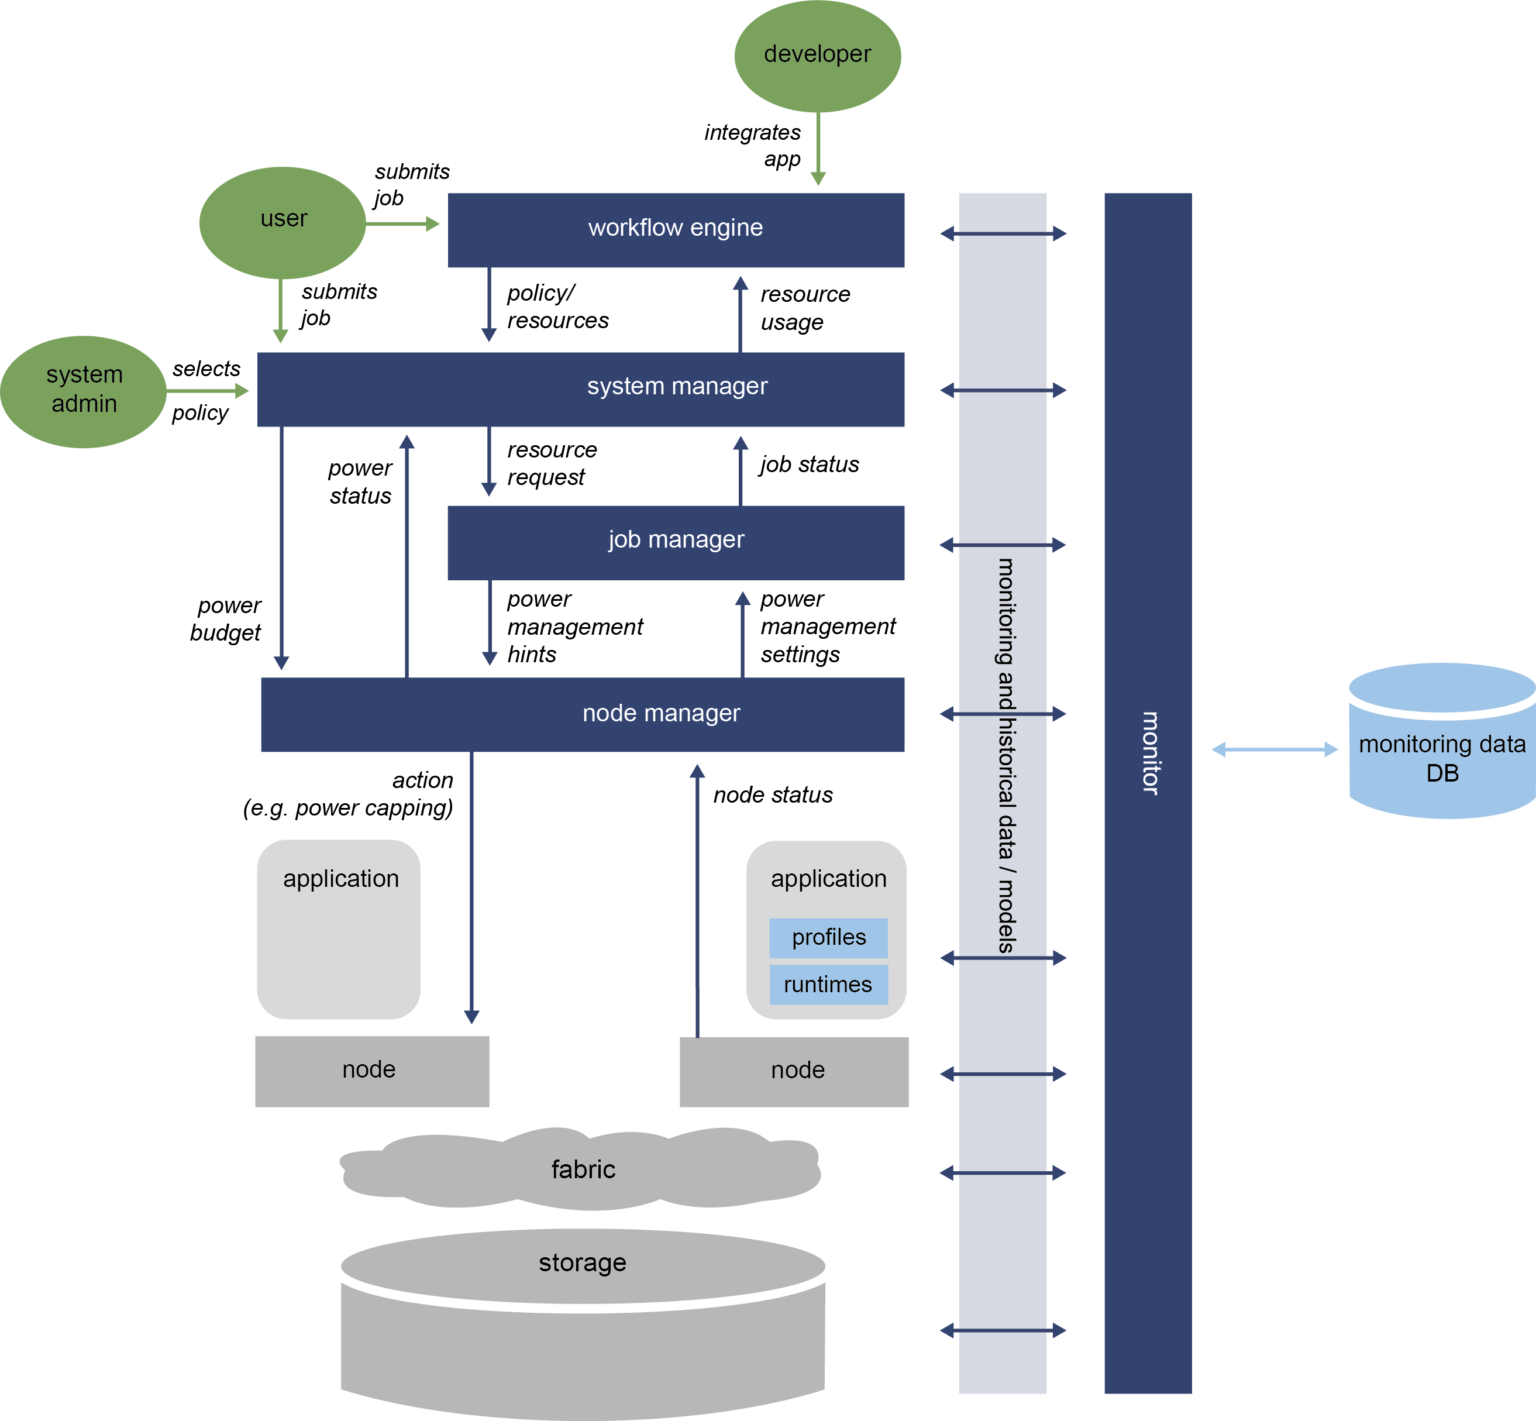
\includegraphics[width=\textwidth]{img/REGALE-Architecture-1536x1421.png}
\end{figure}
\subsection{Workflow engine}
The workflow engine analyses the dependencies and resource requirements of each workflow and decides on how to break the workflow into specific jobs that will be fed to the system manager. 

Job schedulers allow high-performance computing users to efficiently share the computing resources that comprise an HPC system. Users submit batch jobs into one or more batch queues that are defined within the job scheduler. The job scheduler examines the overall set of pending work waiting to run on the computer and makes decisions about which jobs to place next onto the computational nodes within the computer. Generally speaking, the job scheduler attempts to optimize some characteristic such as overall system utilization or fast access to resources for some subset of batch jobs within the computing center's overall workload. The various queues that are defined within the job scheduler may be designated as having higher or lower priorities and may be restricted to some subset of the center's users, thus allowing the job scheduler to understand distinctions of importance of certain jobs within the overall workflow.


\subsection{System Manager}
Receives as input a set of jobs to be scheduled within the system and indicatively decides upon when to schedule each job, to which specific compute nodes to map it, and under which power budget or setting. For this, it constantly monitors and records power and energy telemetry data, and controls power budgets/settings and/or user fairness
%To carry out its work, a job scheduler typically interacts with one or more resource managers. A resource manager is a piece of system software that has privileged ability to control various resources within a datacenter. These resources can include things such as the physical nodes that make up a highperformance computer's computational resources; disks, disk channels, or burst buffer hardware that comprise I/O resources; or network interfaces, network channels, or switches that comprise interconnect resources. For example, a job scheduler might use resource management software to configure the processing cores, memory, disk, and networking resources within one or more computational nodes in accordance with the requested resources for a specific batch job prior to launching that job onto the allocated computational nodes. Finally, in some cases, resource management software might have the ability to actuate pieces of the physical plant that are responsible for delivering electricity to the datacenter or cooling the datacenter

\subsection{Job Manager}
By analysing the profiles, Job Manager decides the target power management knob (CPU power cap, CPU clock frequency scaling or any others) as well as performs code tuning as an option. 

\subsection{Node Manager}
The node manager provides access to node-level hardware controls and monitors. Moreover, the node manager implements processor level and node level power management policies, as well as preserving the power integrity, security and safety of the node. 

\subsection{Monitor}
The monitor is responsible for collecting in-band and out-of-band data for performance, resource utilization, status, power, energy, with minimal footprint, collecting, aggregating, and analysing various metrics, and pushing necessary real-time data to the other entities.
